\chapter{Release 2}
\label{chap:release2}

\section{Introduction}
\label{sec:release2-intro}

Release 2 encompasses the final two sprints of the Production Tracker project, focusing on real-time communication through integrated chat systems, quick identification with QR code technology, intelligent reporting with AI assistance, and comprehensive notification management. This release delivers advanced features that enhance user collaboration, operational visibility, and decision-making capabilities.

\section{Sprint 4: Notes, Real-Time Chat, and Notifications}
\label{sec:sprint4}

\subsection{Sprint Backlog}
\label{sec:sprint4-backlog}
the table \ref{tab:sprint4-backlog} summarizes the user stories and tasks completed during Sprint 4:
\footnotesize
\begin{longtable}{|p{0.10\textwidth}|p{0.50\textwidth}|p{0.32\textwidth}|}
    \caption{Sprint 4 Backlog}\label{tab:sprint4-backlog}\\
    \hline
    \textbf{ID} & \textbf{User Story} & \textbf{Tasks} \\
    \hline
    \endfirsthead
    \hline
    \textbf{ID} & \textbf{User Story} & \textbf{Tasks} \\
    \hline
    \endhead
    \hline
    \endfoot
    PB-11 & As a worker, I want to add notes on work stages so that operational details are documented. & Create notes logic; \newline  Build notes UI; \newline  Add note timestamp and author tracking \\
    \hline
    PB-12 & As a user, I want to chat with other users in real time so that I can discuss issues. & Setup real-time communication; \newline  Build chat interface; \newline  Implement message history \\
    \hline
    PB-13 & As a user, I want to attach files in chat so that I can share documents and evidence. & Build file upload handler; \newline   Add file attachment UI \\
    \hline
    PB-14 & As a user, I want to receive notifications so that I do not miss important events. & Implement notification service; \newline  Build notification UI; \newline  Add notification management \\
    \hline
\end{longtable}
\normalsize

\subsection{Sprint 4 Use Case Diagram}
the figure \ref{fig:sprint4-use-case-diagram} illustrates the main use cases implemented in Sprint 4, focusing on real-time communication and notification features. It shows the interactions between users for adding notes, engaging in chat conversations, attaching files, and managing notifications within the system.
\begin{figure}[H]
    \centering
    
    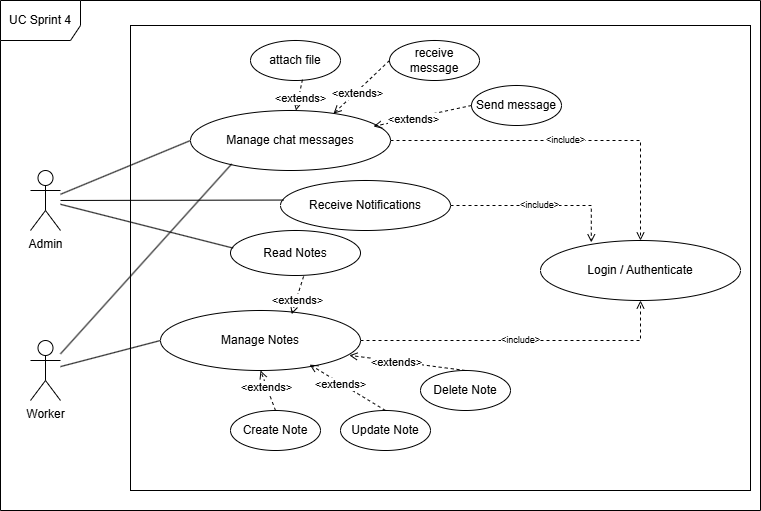
\includegraphics[width=\textwidth,keepaspectratio]{pictures/Sprint 4 UC Diagram.drawio.png}
    \vspace*{\fill}
    \caption{Sprint 4 Use Case Diagram}
    \label{fig:sprint4-use-case-diagram}
\end{figure}
\vspace{1cm}
\subsection{Sequence Diagram for Real-Time Messaging}
the figure \ref{fig:real-time-chat-sequence-diagram} illustrates the sequence of interactions that occur during a real-time chat session between two users. It shows how messages are sent, received, and persisted in the system, highlighting the use of Socket.IO for real-time communication and the integration with the database for message storage.
\begin{sidewaysfigure}
    \centering
    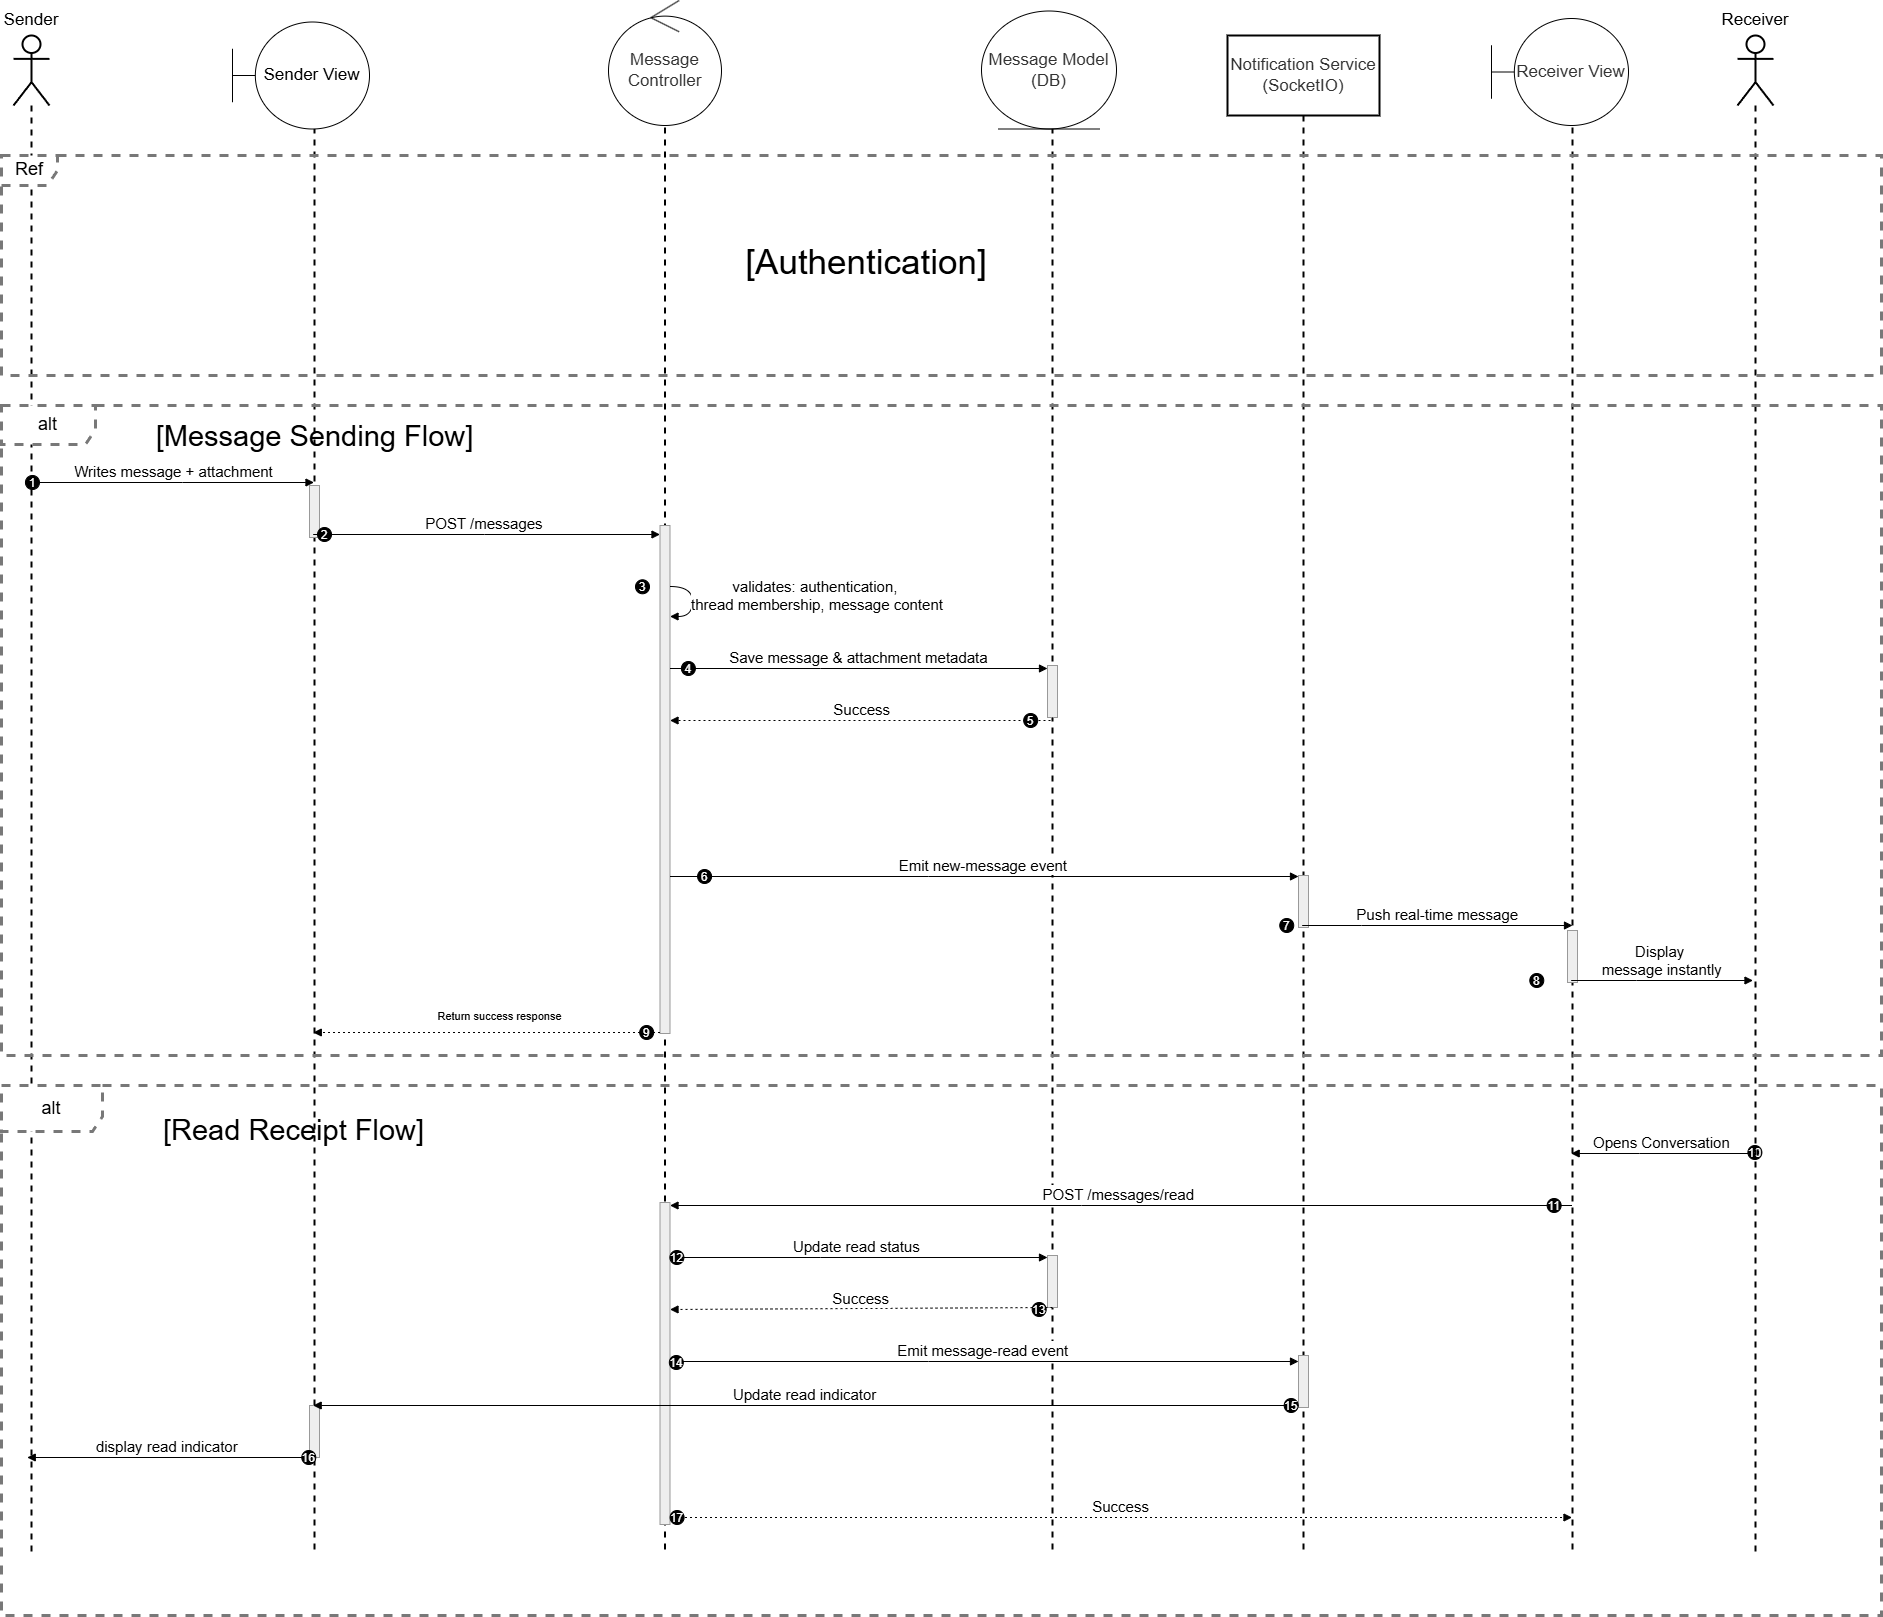
\includegraphics[width=0.8\textheight]{pictures/Real-time chat message flow.drawio.png}
    \caption{Real-Time Chat Message Flow Sequence Diagram}
    \label{fig:real-time-chat-sequence-diagram}
\end{sidewaysfigure}
\vspace{1cm}
\subsection{Sprint 4: Application Interface Overview}

\label{sec:sprint4-interfaces}
the figures \ref{fig:note-management-worker}, \ref{fig:notes-history-admin} illustrate the note management interfaces for workers and administrators, respectively. The worker view allows users to add and view notes related to their tasks, while the admin view provides a comprehensive history of all notes for monitoring and analysis.
\begin{figure}[H]
    \centering

    \begin{minipage}[t]{0.48\textwidth}
        \centering
        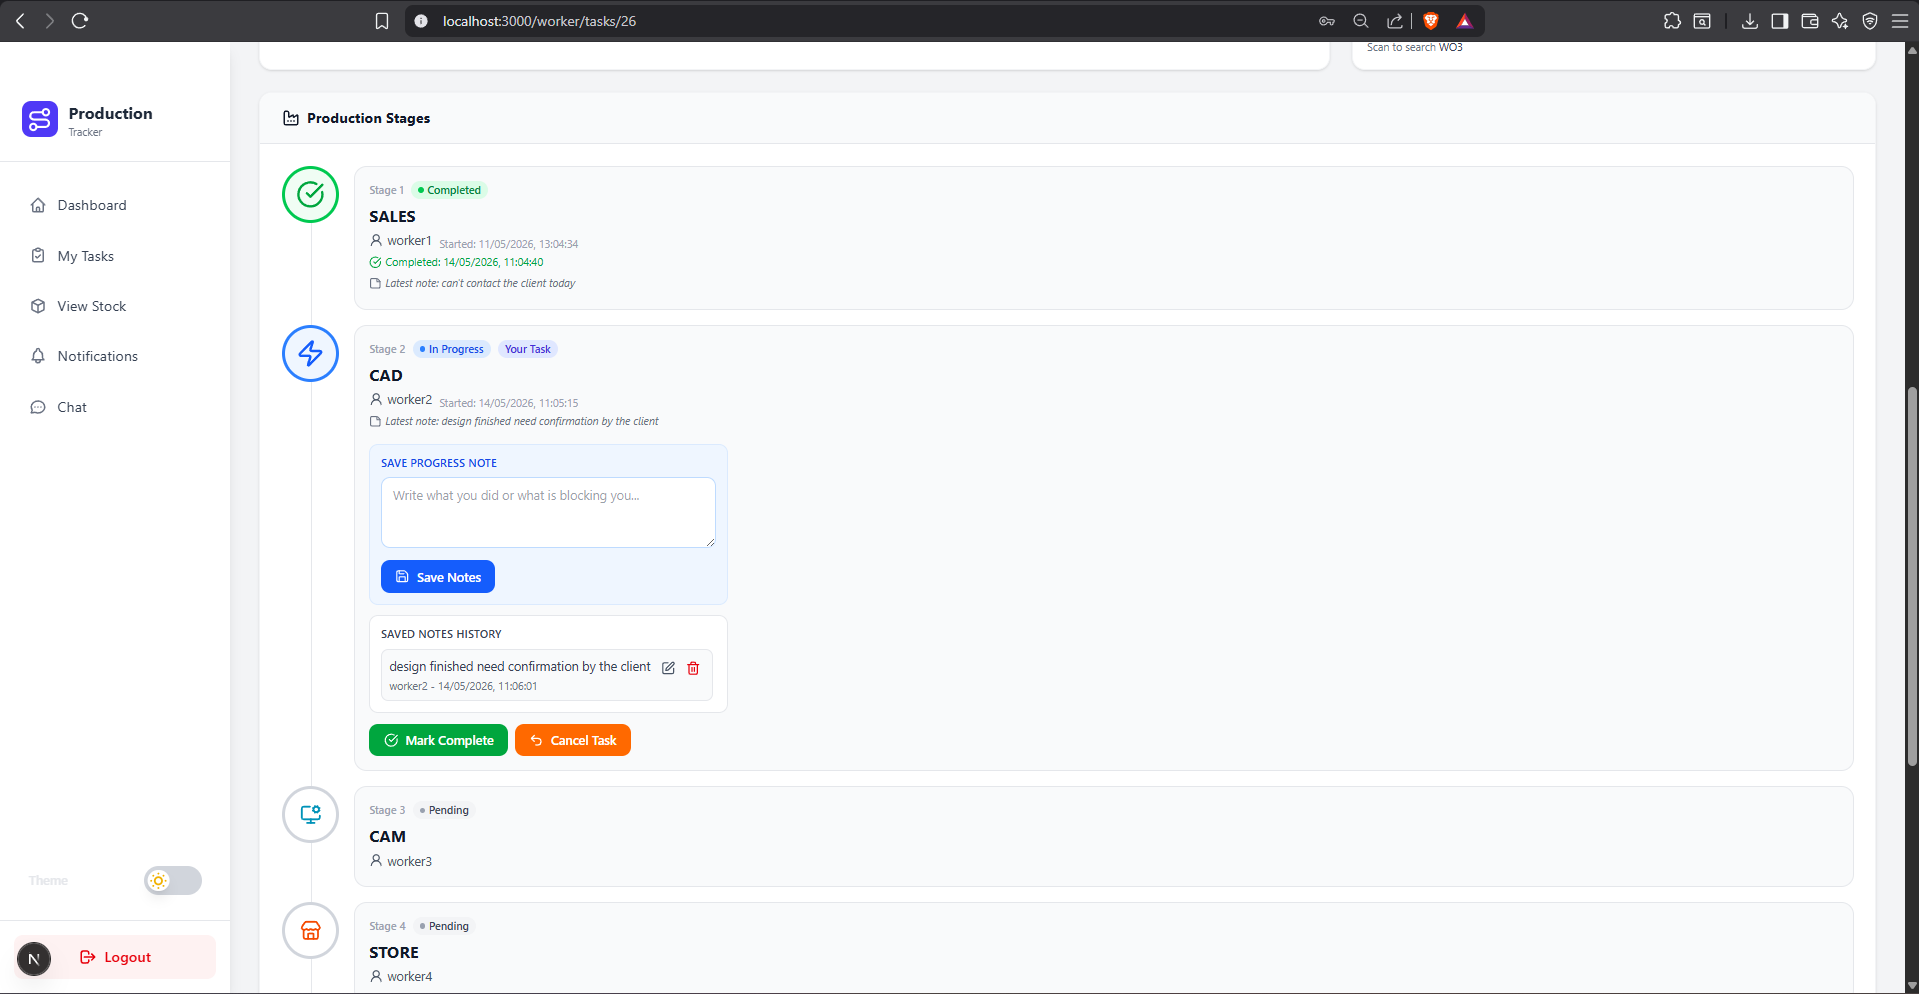
\includegraphics[width=\textwidth,keepaspectratio]{pictures/note managment worker view.png}
        \caption{Note Management Worker View}
        \label{fig:note-management-worker}
    \end{minipage}
    \hfill
    \begin{minipage}[t]{0.48\textwidth} 
        \centering
        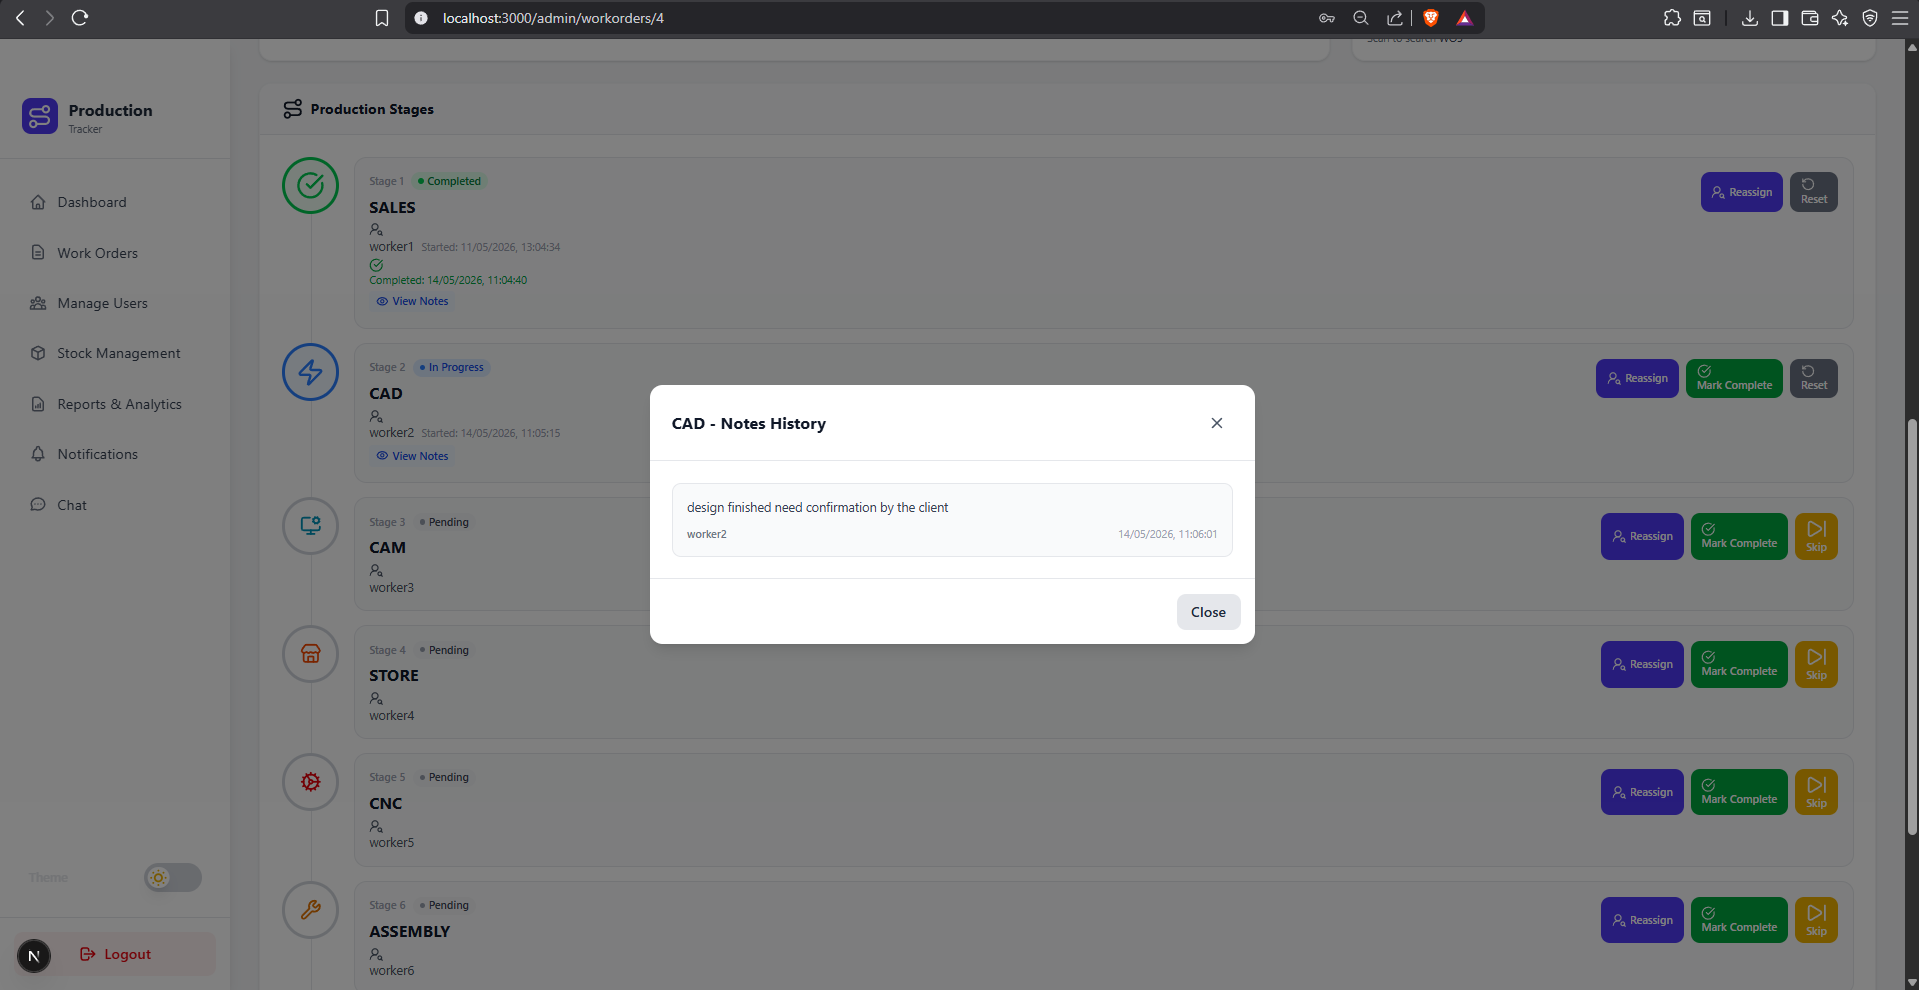
\includegraphics[width=\textwidth,keepaspectratio]{pictures/notes history admin view.png}
        \caption{Notes History Admin View}
        \label{fig:notes-history-admin}
    \end{minipage}

\end{figure}

the figures \ref{fig:chat-messaging-worker} and \ref{fig:chat-messaging-admin} provide an overview of the real-time chat messaging interfaces.
\begin{figure}[H]
    \centering

    \begin{minipage}[t]{0.48\textwidth}
        \centering
        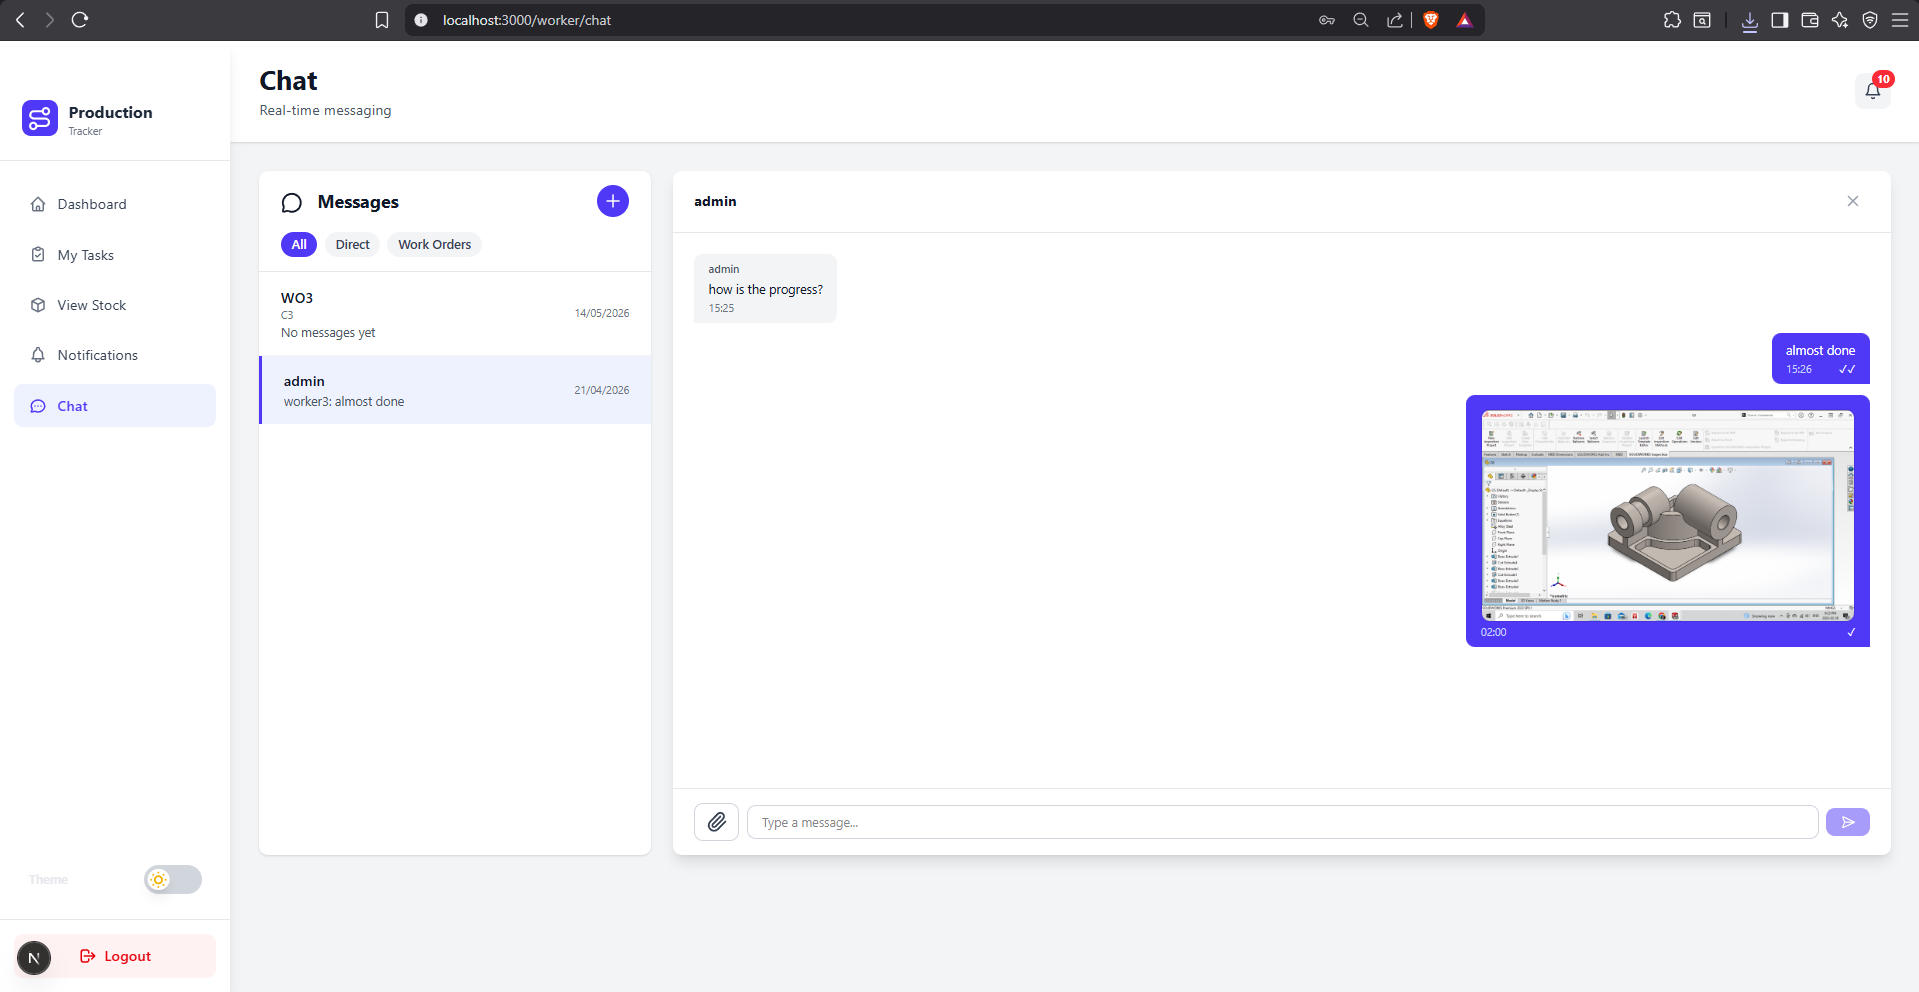
\includegraphics[width=\textwidth,keepaspectratio]{pictures/chat messaging interface worker view.png}
        \caption{Chat Messaging Interface Worker View}
        \label{fig:chat-messaging-worker}
    \end{minipage}
    \hfill
    \begin{minipage}[t]{0.48\textwidth} 
        \centering
        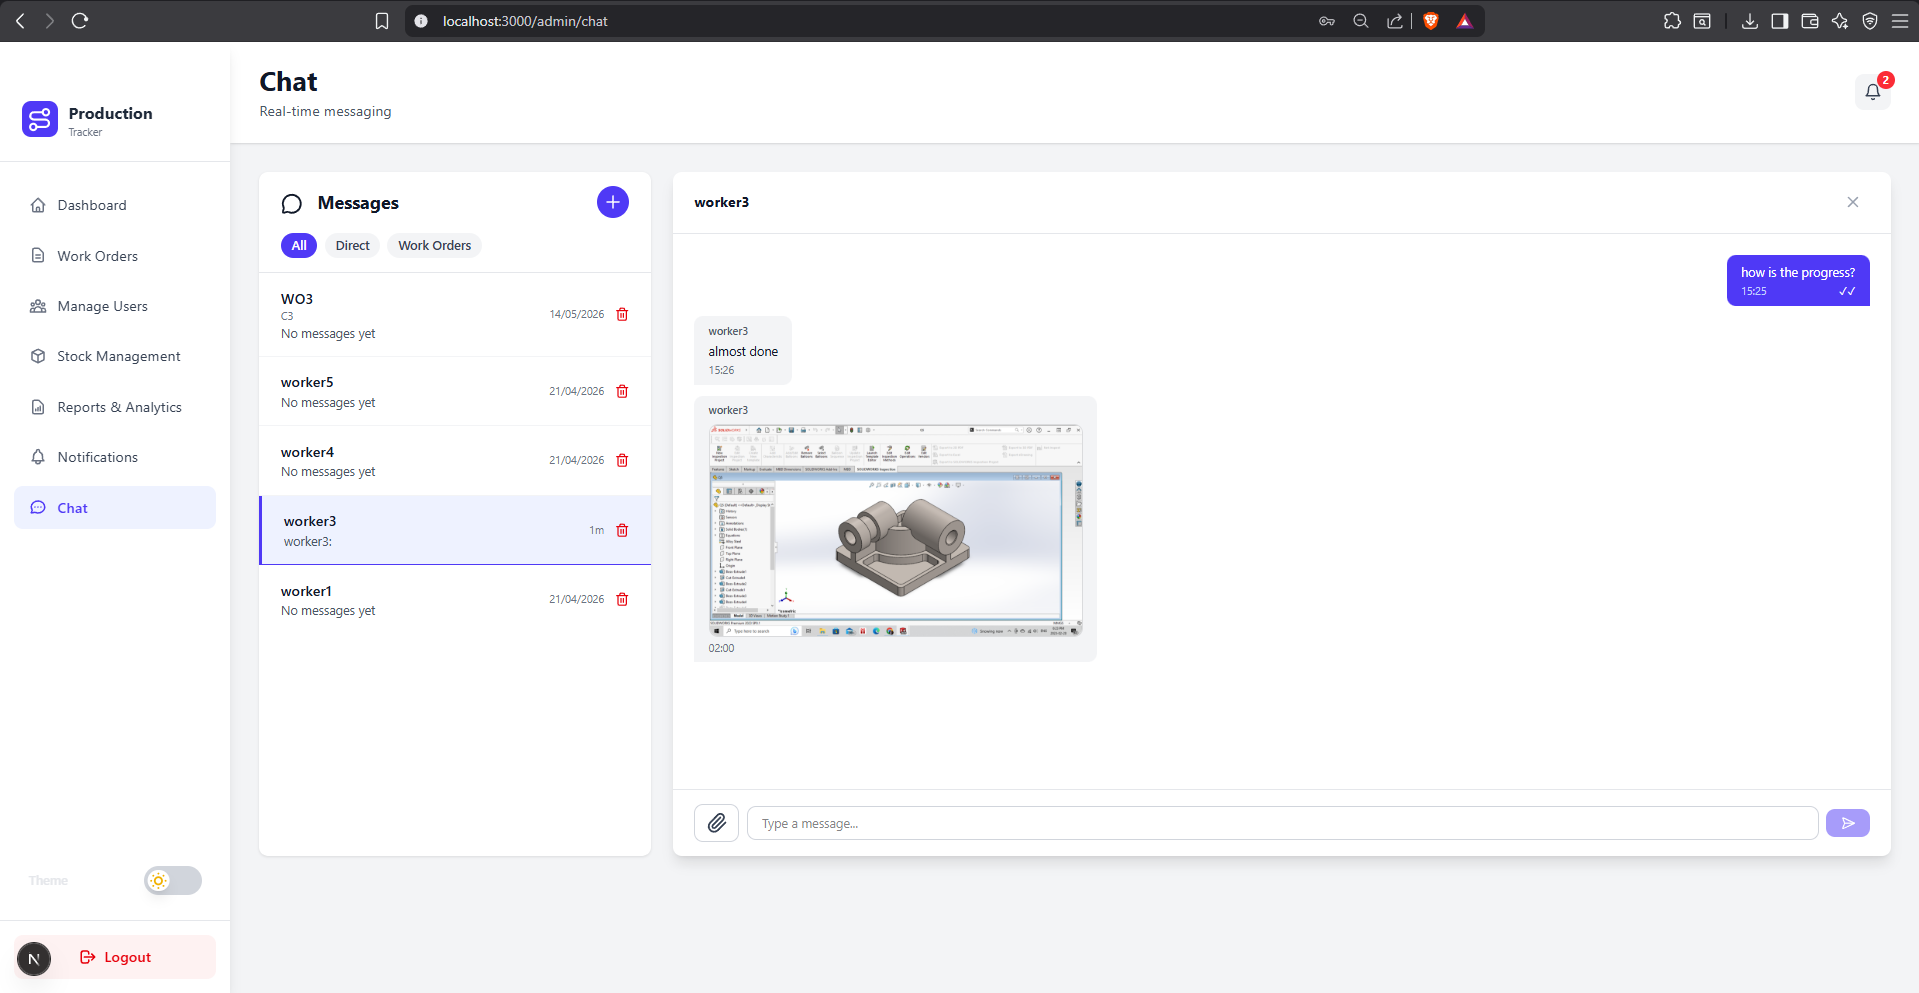
\includegraphics[width=\textwidth,keepaspectratio]{pictures/chat messaging admin view.png}
        \caption{Chat Messaging Interface Admin View}
        \label{fig:chat-messaging-admin}
    \end{minipage}

\end{figure}
the figure \ref{fig:notification-center} illustrates the notification center interface for managing alerts and notifications within the system.
\begin{figure}[H]
    \centering
\begin{minipage}[t]{0.48\textwidth} 
        \centering
        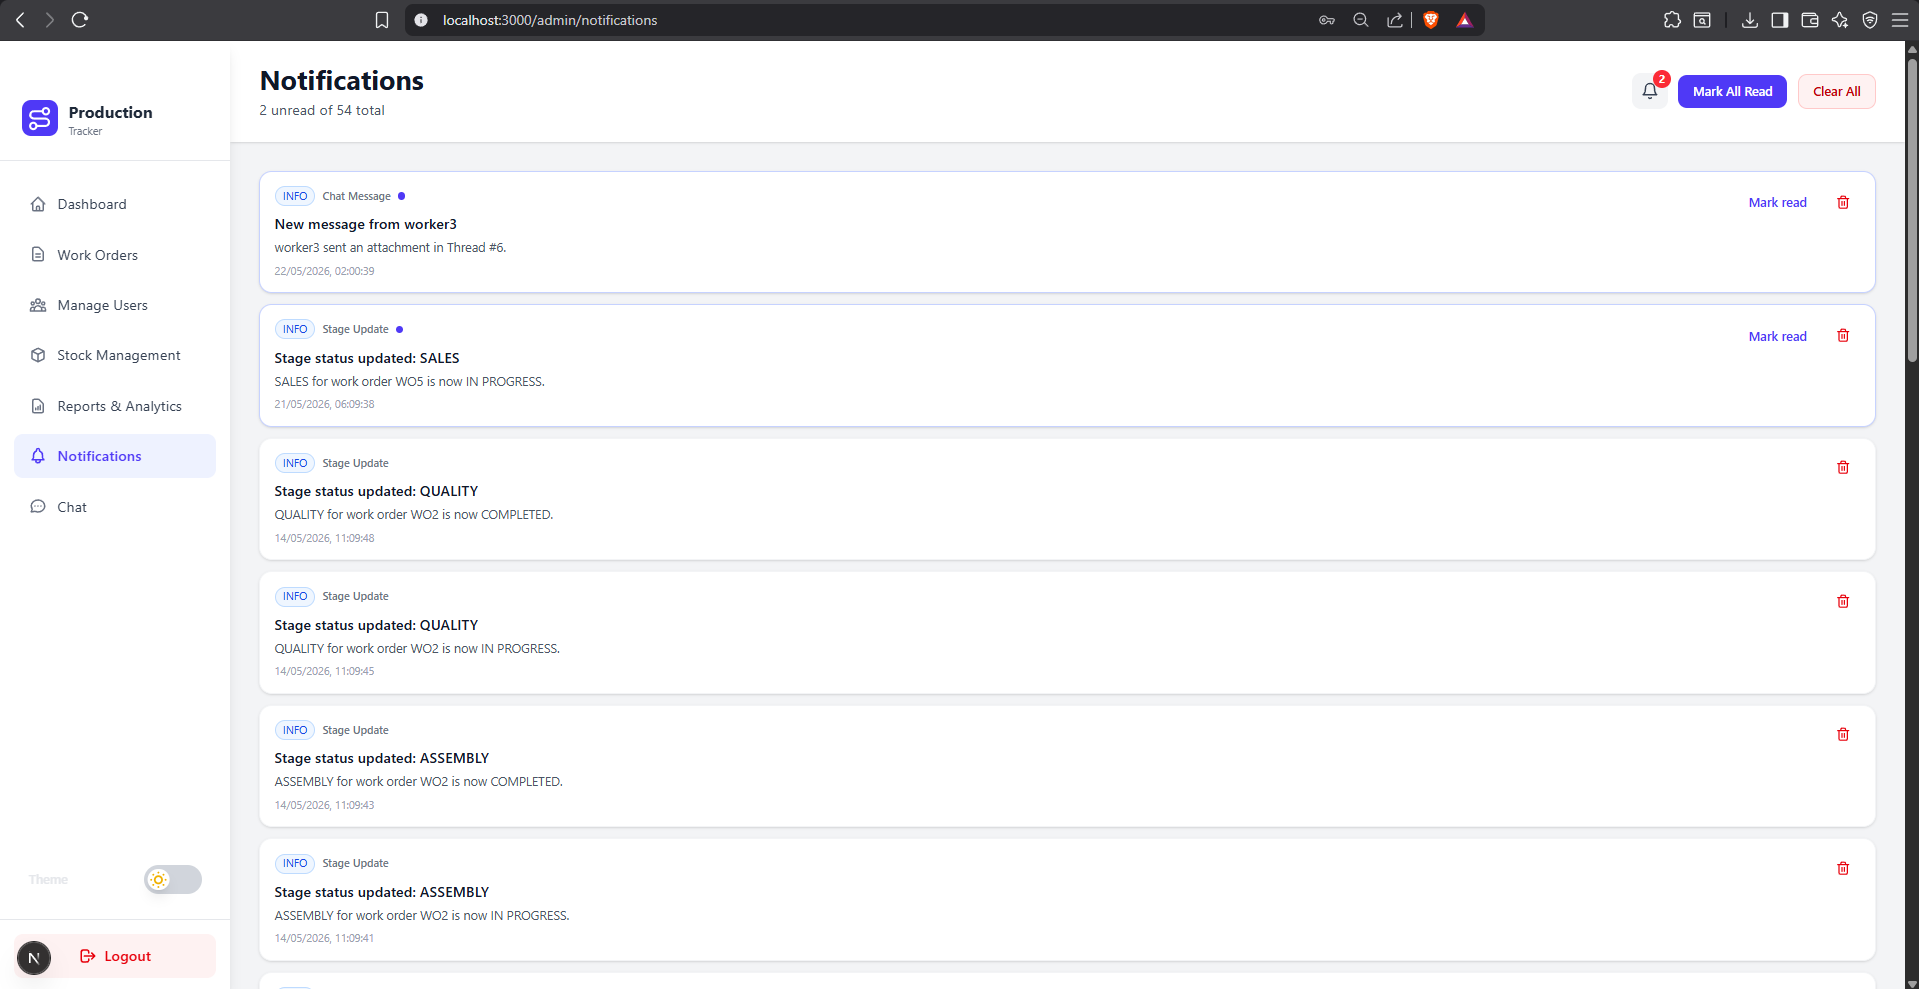
\includegraphics[width=\textwidth,keepaspectratio]{pictures/notification center.png}
        \caption{Notification Center}
        \label{fig:notification-center}
    \end{minipage}
\end{figure}
\section{Sprint 5: QR Codes, Analytics, and AI Reporting}
\label{sec:sprint5}

\subsection{Sprint Backlog}
\label{sec:sprint5-backlog}
the table \ref{tab:sprint5-backlog} summarizes the user stories and tasks completed during Sprint 5:

\footnotesize
\begin{longtable}{|p{0.10\textwidth}|p{0.50\textwidth}|p{0.32\textwidth}|}
    \caption{Sprint 5 Backlog}\label{tab:sprint5-backlog}\\
    \hline
    \textbf{ID} & \textbf{User Story} & \textbf{Tasks} \\
    \hline
    \endfirsthead
    \hline
    \textbf{ID} & \textbf{User Story} & \textbf{Tasks} \\
    \hline
    \endhead
    \hline
    \endfoot
    PB-15 & As an administrator, I want generated QR codes for work orders so that identification is faster. & Implement QR code library; \newline  Build generation API; \newline  Add QR display  \\
    \hline
    PB-16 & As a user, I want to scan QR codes so that I can quickly search and access work orders . & Integrate QR scanner; \newline  Build scan interface; \newline  Add scan result handler \\
    \hline
    PB-17 & As an administrator, I want AI-assisted reporting so that I can make faster decisions. & Setup reporting engine; \newline  Integrate AI analysis; \newline  Build dashboard UI \\
    \hline
    PB-18 & As an administrator, I want a analytical dashboard for the production data. & Build analytics UI; \newline  Integrate data visualization; \\
    \hline
\end{longtable}
\normalsize

\subsection{Sprint 5 Use Case Diagram}
\label{sec:sprint5-use-case-diagram}
the figure \ref{fig:sprint5-use-case-diagram} illustrates the main use cases implemented in Sprint 5:
\begin{figure}[H]
    \centering
    
    \includegraphics[width=0.8\textwidth,
    height=0.6\textheight,
    keepaspectratio]{pictures/Sprint 5 UC Diagram.drawio.png}
    \vspace*{\fill}
    \caption{Sprint 5 Use Case Diagram}
    \label{fig:sprint5-use-case-diagram}
\end{figure}

\subsection{Sequence Diagram for AI-Based Report Generation}
\label{sec:sprint5-sequence-diagram}
the figure \ref{fig:sprint5-sequence-diagram} illustrates the sequence of interactions that occur during the AI-based report generation process. It shows how data is collected, processed, and analyzed using AI to generate insightful reports for administrators.
\begin{figure}[H]
    \centering
    
    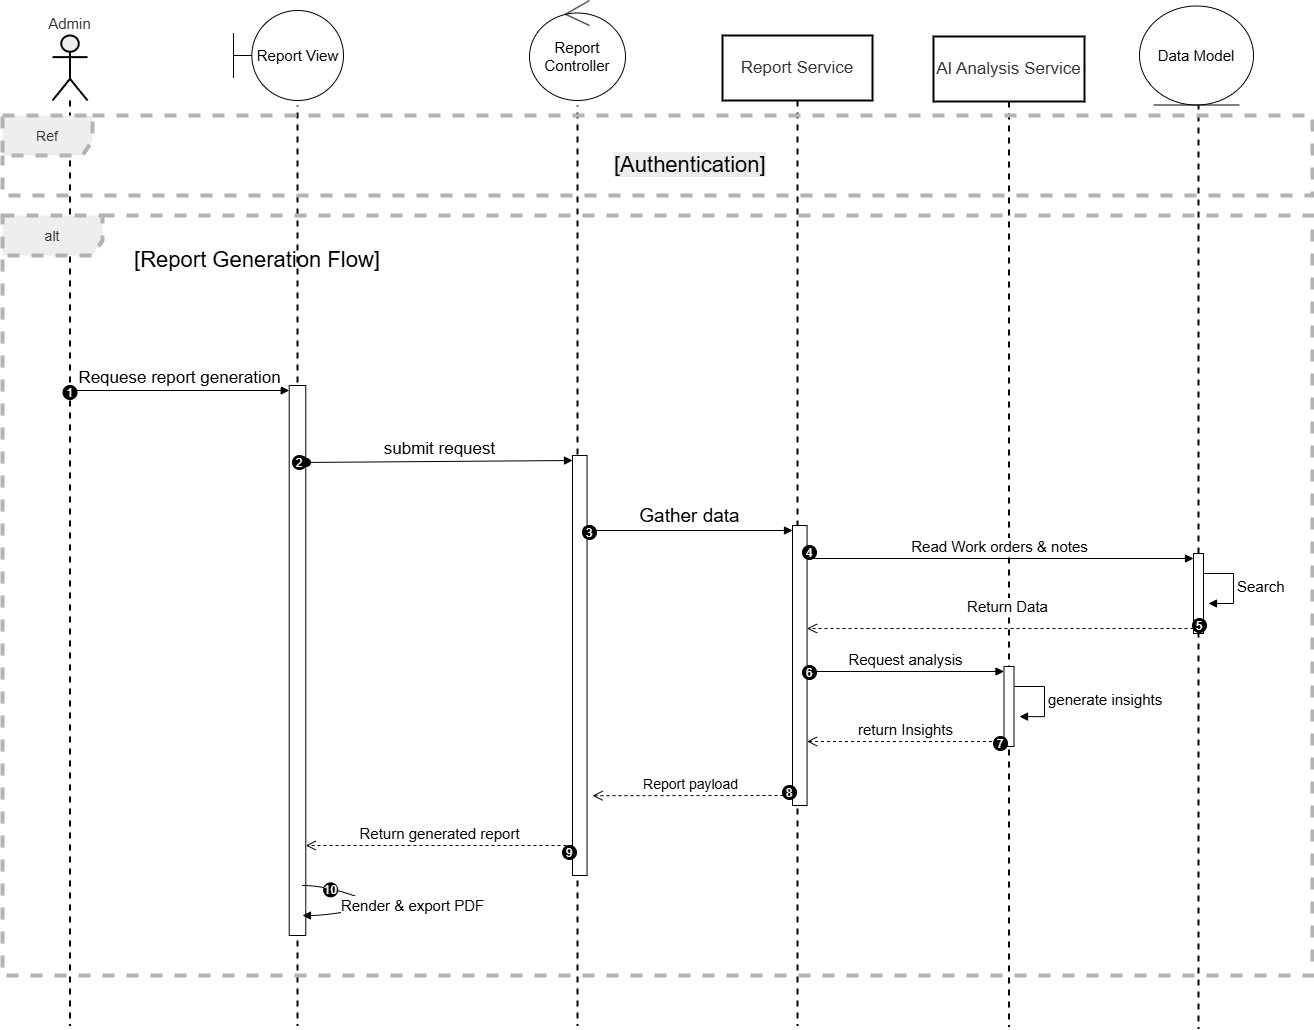
\includegraphics[width=\textwidth,
    height=0.6\textheight,
    keepaspectratio]{pictures/AI report sequence diagram.drawio.png}
    \vspace*{\fill}
    \caption{Sequence Diagram for AI-Based Report Generation}
    \label{fig:sprint5-sequence-diagram}
\end{figure}

\subsection{Sprint 5: Application Interface Overview}
the figures \ref{fig:workorder-details-with-qr} and \ref{fig:qr-code-scanner} illustrate the interfaces for work order details with QR code display and the QR code scanner, respectively. The work order details interface allows users to view comprehensive information about a work order along with a generated QR code for quick access, while the QR code scanner interface enables users to scan codes and retrieve associated work order information efficiently.
\begin{figure}[H]
    \centering

    \begin{minipage}[t]{0.48\textwidth}
        \centering
        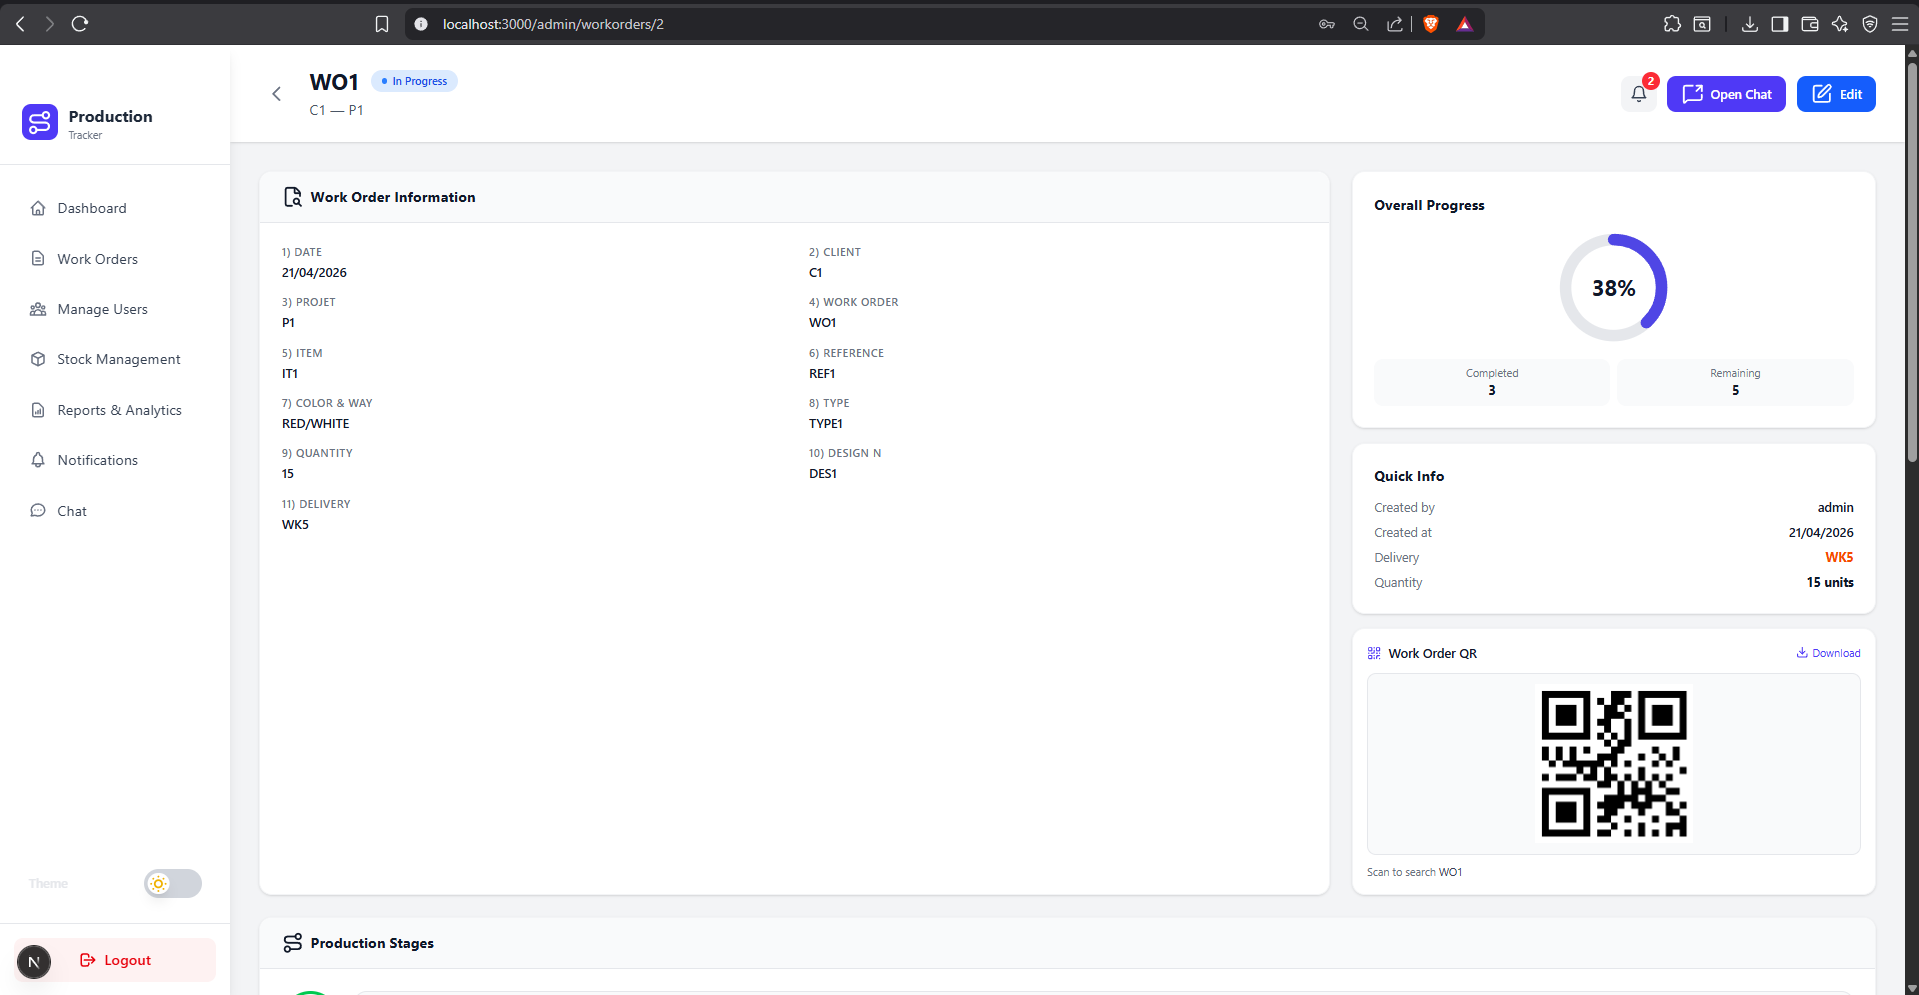
\includegraphics[width=\textwidth,keepaspectratio]{pictures/workorder detailes interface with QR code.png}
        \caption{Work Order Details Interface with QR Code}
        \label{fig:workorder-details-with-qr}
    \end{minipage}
    \hfill
    \begin{minipage}[t]{0.48\textwidth} 
        \centering
        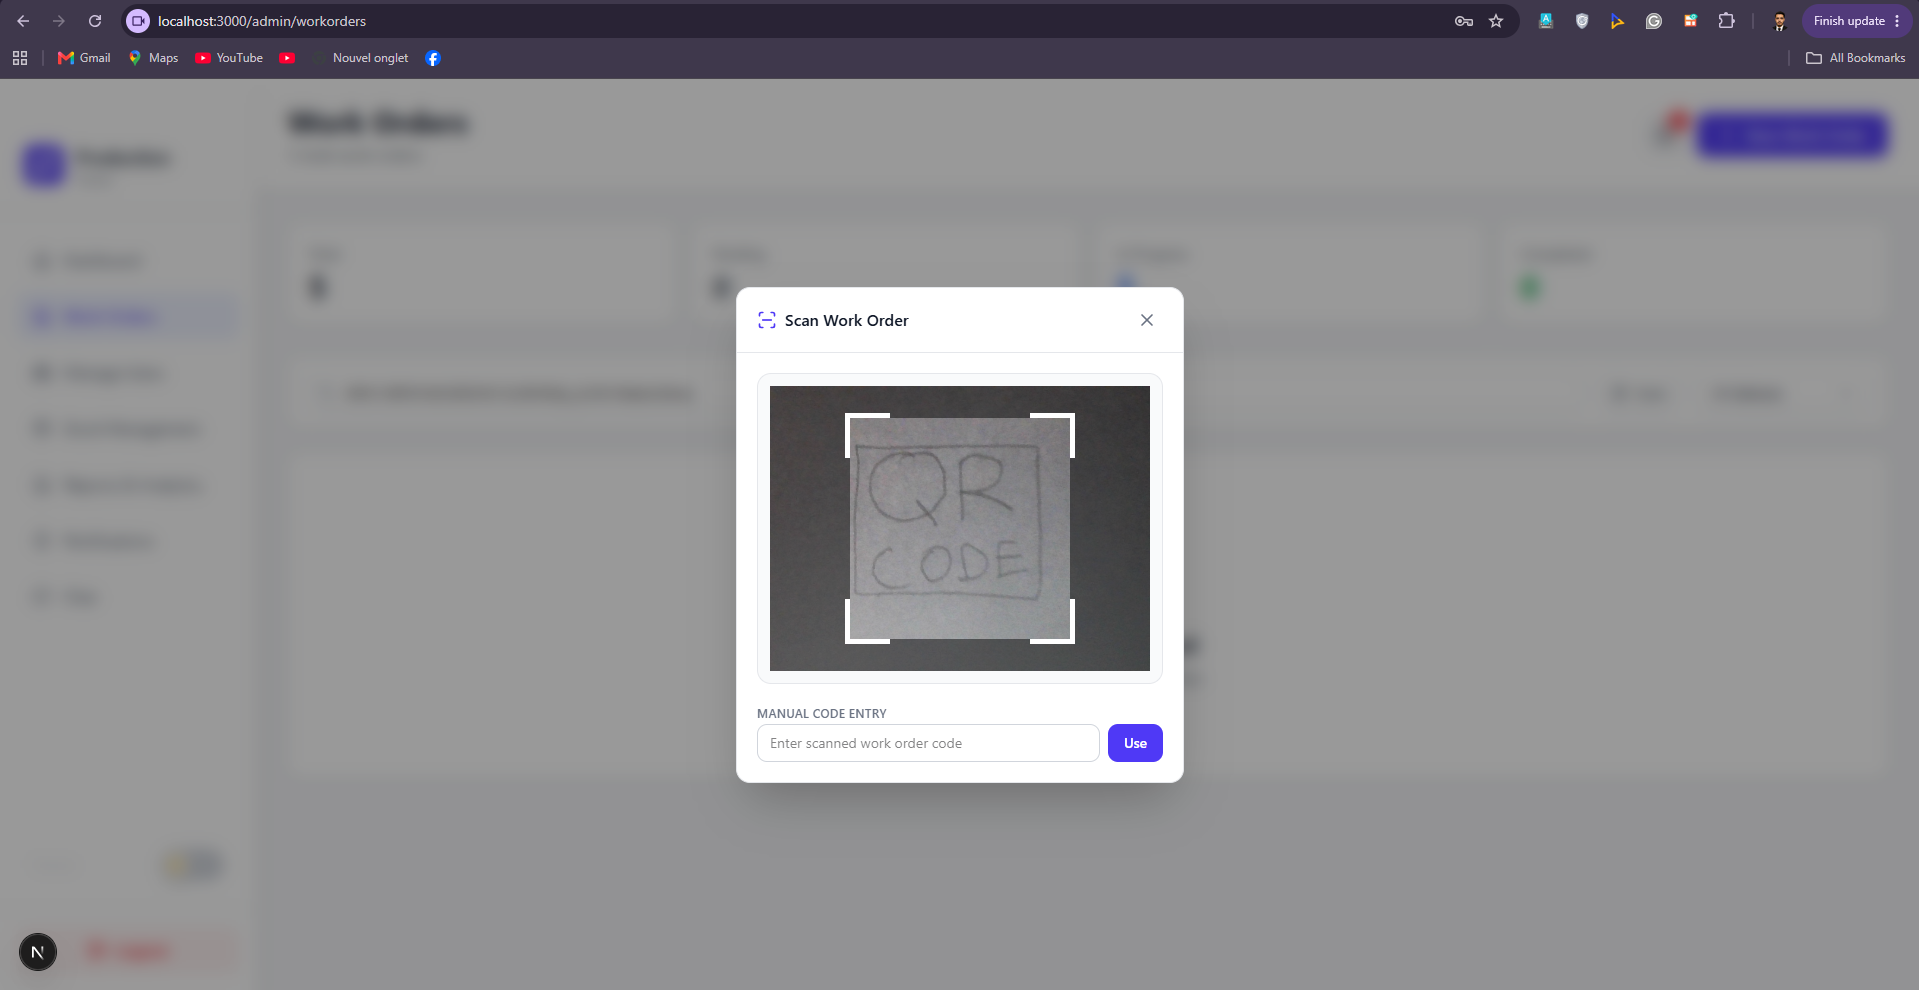
\includegraphics[width=\textwidth,keepaspectratio]{pictures/Qr code scanner interface.png}
        \caption{QR Code Scanner Interface}
        \label{fig:qr-code-scanner}
    \end{minipage}

\end{figure}
the figures \ref{fig:ai-report-interface} and \ref{fig:analytics-dashboard} provide an overview of the AI report interface and the analytics dashboard, respectively. The AI report interface allows administrators to generate and view AI-assisted reports, while the analytics dashboard provides visualizations and insights based on production data for informed decision-making.
\begin{figure}[H]
    \centering

    \begin{minipage}[t]{0.48\textwidth}
        \centering
        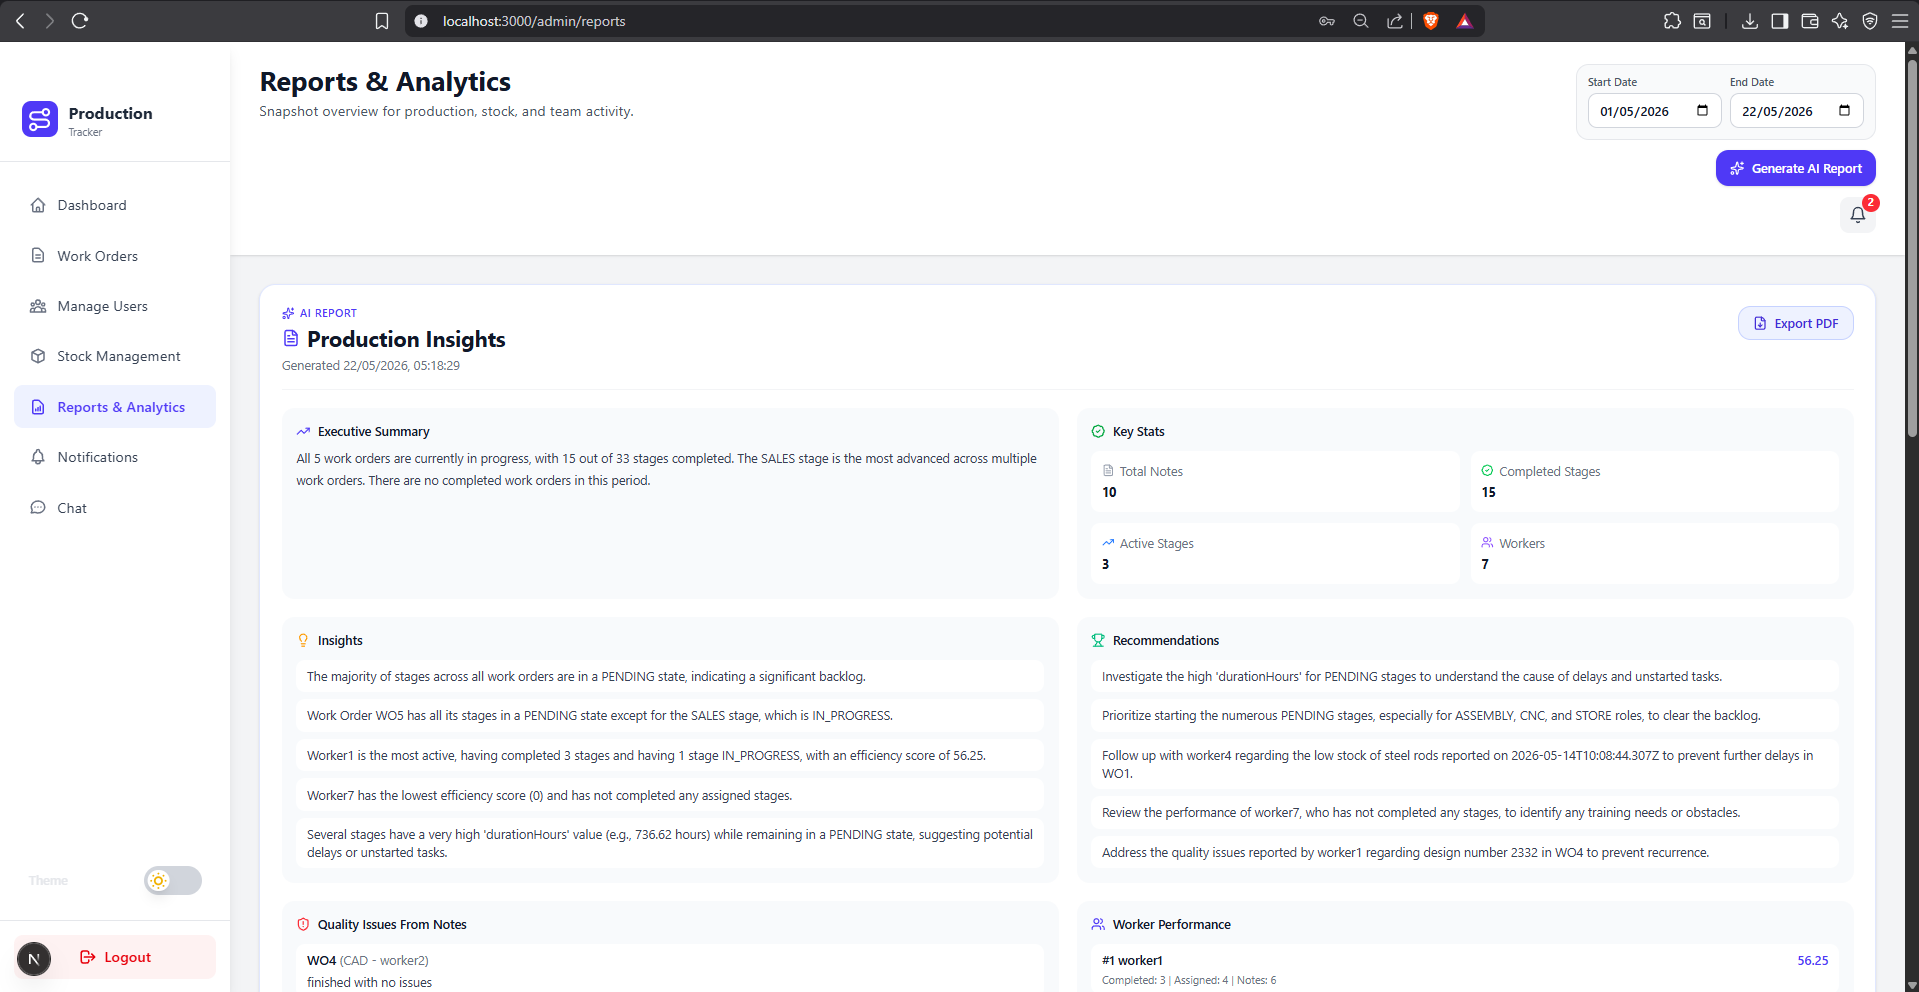
\includegraphics[width=\textwidth,keepaspectratio]{pictures/Ai report interface.png}
        \caption{AI Report Interface}
        \label{fig:ai-report-interface}
    \end{minipage}
    \hfill
    \begin{minipage}[t]{0.48\textwidth}
        \centering
        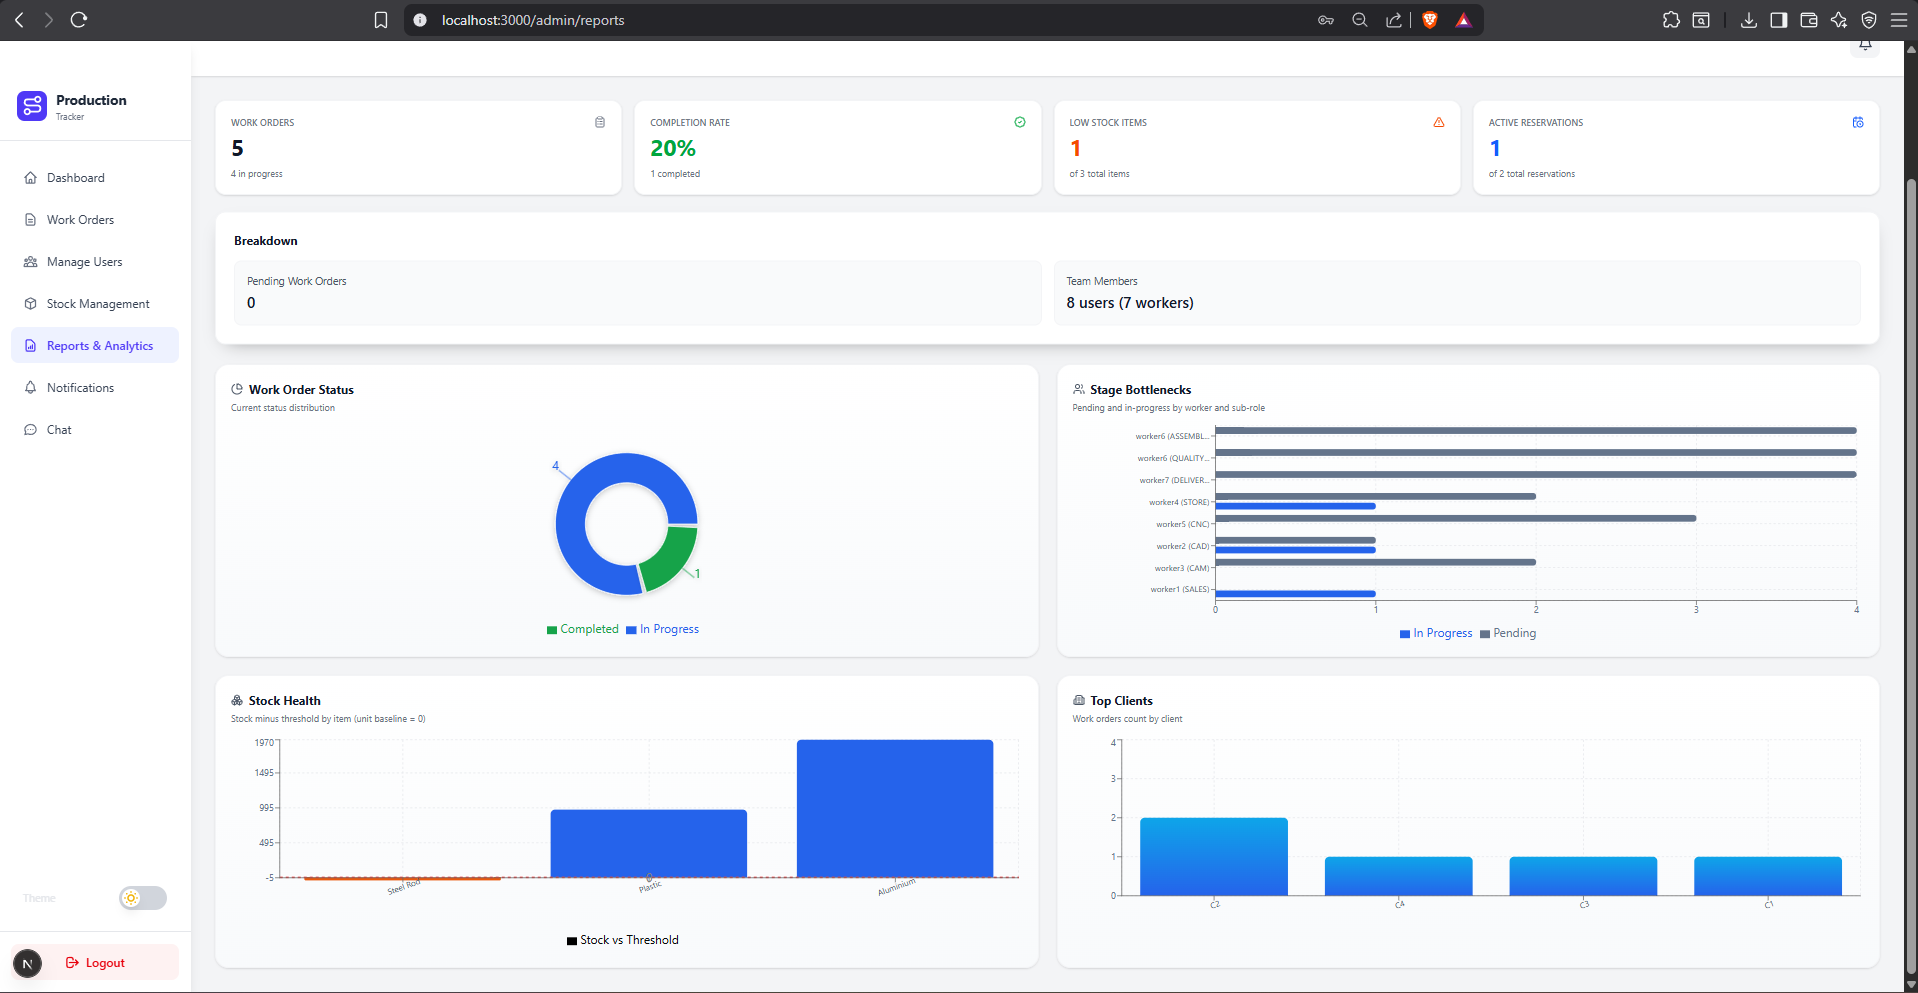
\includegraphics[width=\textwidth,keepaspectratio]{pictures/analytics Dashboard.png}
        \caption{Analytics Dashboard}
        \label{fig:analytics-dashboard}
    \end{minipage}

\end{figure}

\label{sec:sprint5-interfaces}

\section{Conclusion}
\label{sec:release2-conclusion}

Release 2 proved to be successful since it provided advanced functionalities that converted the Production Tracker into a fully-featured collaboration tool. The two sprints in Release 2 took 21 days each (summing up to 42 days), incorporating real-time communication features, effective identifying methods, and intelligent reporting. Combining Release 2 with Release 1 made up the 5-sprint process taking a total of 105 days to develop the application.
